\documentclass[11pt]{article}

\usepackage{cite}
\usepackage{graphicx}
\usepackage{hyperref}

\hypersetup{colorlinks=true, linkcolor=blue}
\def\UrlBreaks{\do/\do-}

\begin{document}

\title{X509 certificates and Certification Authorities\\ HW5 - CNS Sapienza}
\author{Davide Spallaccini - 1642557}
\date{26 of November 2017}
\maketitle

\section{Introduction}
In this work we will review the basics of digital certificates and Certification Authorities. Digital certificates are digital files whose purpose is to certify the identity of individuals or institutions dealing with internet-based information. Certifications Authorities are the institutions that are charged to issue these certificates. In the following sections we will describe how to retrive and read the certificates available to some commonly used browsers and supply further informations about CAs and the X.509 public key infrastructure and certificate chains, with a special reference to the macOS operating system.

\section{X.509 certificates and Certification Authorities: a review}
The problem of encryption alone is that it provides not enough security as it provides no proof of the identity of the sender of encrypted information. A certificate, also known as a “digital certificate” or a “public key certificate,” is a file that together with encryption helps keep web communications secure assuring the identity of all the parties involved in a transaction. An encrypted website and a particular browser work together to make the communication secret by means of encryption. The key for such encryption is contained in the certificate. Usually is it possible for users to install new certificates for authenticating to some given websites.

X.509 is a standard that defines the format of these certificates. The main content of the certificate is a public key for some asymmetric encryption algorithm and an identity, in the form of a hostname or organization name. The key security advantage of certificates is that when a certificate is signed by a trusted Certification Authority, or validated by other means, someone holding that certificate can rely on the public key it contains to establish secure communications with another party, or validate documents digitally signed by the corresponding private key.

The main contents of a certificate are the following \cite{mozillasupport}:
\begin{itemize}
\item Serial Number: Uniquely identifies the certificate.
\item Subject: Identifies the certificate owner, such as the name of the organization owning the certificate.
\item Issuer: Identifies the entity that issued the certificate.
\item Subject Alt Name Extension: List of website addresses that the certificate can be used to identify.
\item Signature: Data that verifies that the certificate came from the Issuer.
\item Signature Algorithm: Algorithm used to create the Signature.
\item Valid-From: The date the certificate is first valid.
\item Valid-To: The expiration date.
\item Key-Usage and Extended Key Usage: Specifies how the certificate may be used, such as for confirming ownership of a website (Web Server Authentication).
\item Public Key: The public part of the data that comprises the public/private key pair.
\item Public Key Algorithm: Algorithm used to create the Public Key.
\item Certificate Signature Algorithm: Algorithm used to create the Fingerprint.
\item Certificate Signature: An abbreviated form of the Public Key.
\end{itemize}

We want to mention here that in the X.509 version 3 standard defines a number of certificate extensions which in general indicate how the certificate should be used. Extensions can be marked as \textit{critical} or \textit{non critical}, and usually most of them are non critical, except for the extension \textit{Key Usage} which is almost always critical: in fact the key usage extension defines the purpose (e.g., encipherment, signature, certificate signing) of the key contained in the certificate. The usage restriction might be employed when a key that could be used for more than one operation is to be restricted.

There are several commonly used filename extensions for X.509 certificates. Unfortunately, some of these extensions are also used for other data such as private keys. A very useful tool the creation of X.509 certificates, CSRs and CRLs files is given by the \texttt{openssl} command line tool with the option \texttt{x509}. We can see the supported and most commonly used file extensions from the tool's usage output:
\begin{verbatim}
usage: x509 args
 -inform arg     - input format, default PEM (one of DER, NET or PEM)
 -outform arg    - output format, default PEM (one of DER, NET or PEM)
 -keyform arg    - private key format - default PEM
 -CAform arg     - CA format - default PEM
 -CAkeyform arg  - CA key format - default PEM
 -in arg         - input file - default stdin
 -out arg        - output file - default stdout
 -passin arg     - private key password source
 -serial         - print serial number value
 -text           - print the certificate in text form
 ...
\end{verbatim}
In particular you can decode a PEM encoded file with extension .crt with the following command \texttt{openssl x509 -in certfilename.crt -text -noout} (we don't present an example output here since it is straightforward, and has the structure of the fields described above). On macOS system the tool can be installed via Homebrew with the command \texttt{brew install openssl}, or you have it already installed if you are using the Anaconda data analytics Python distribution and package management system.

\paragraph*{Certification Authorities and certificate chains}
The main task of Certification Authorities is the one of embedding the public key of an organization or individual along with other identifying information into each digital certificate. After doing so, to guarantee the validity and integrity of these files, the CAs cryptographically sign the documents as a tamper-proof seal. It is possible that the user of a public key found in a certificate does not have a copy of the public key of the CA that signed the certificate itself. So the user needs another certificate to obtain such a public key. In general, a chain of multiple certificates may be needed, such chains are also called certificates paths in the RFC 5280\cite{rfc5280 }. The last certificate in the list is a \textit{trust anchor}: a certificate that you trust because it was delivered to you by some trustworthy procedure. The validation process that traverses one of the possible paths has actually to also take into account additional checks like dates validity and CRLs lookups. At this point X.509 certificates can be classified in three high level categories: end-entity certificates, the ones identified by the browsers; intermediate certificates, used to sign end-entity certificate; and root certificates, which have the characteristic of being self-signed, in the sense that their signature can be validated with the same public key in the certificate. In fact these certificates represent the Certification Authority itself, and have the same organization in the issuer and subject fields.

Worldwide, the certificate authority business is fragmented, with national or regional providers dominating their home market. This is because many uses of digital certificates, such as for legally binding digital signatures, are linked to local law, regulations, and accreditation schemes for certificate authorities.

\paragraph*{Italian Certification Authorities}
In Italy the AgID institution, a public agency under the power and watch of the Prime Minister, aimed at pursuing the maximum technological innovation degree in the development of public administration, provides an official list of active and dismissed Italian Certification Authorities which is published at the following \href{http://www.agid.gov.it/identita-digitali/firme-elettroniche/certificatori-attivi}{link}.

\section{Certificates management in macOS browsers}
The browser you're using right now trusts a bunch of certificate authorities. Which bunch of certificate authorities - properly called a \textit{root certificate store} - is determined by your OS and browser, as shown in Figure\ref{fig:rootstores}.

\begin{figure}[h]
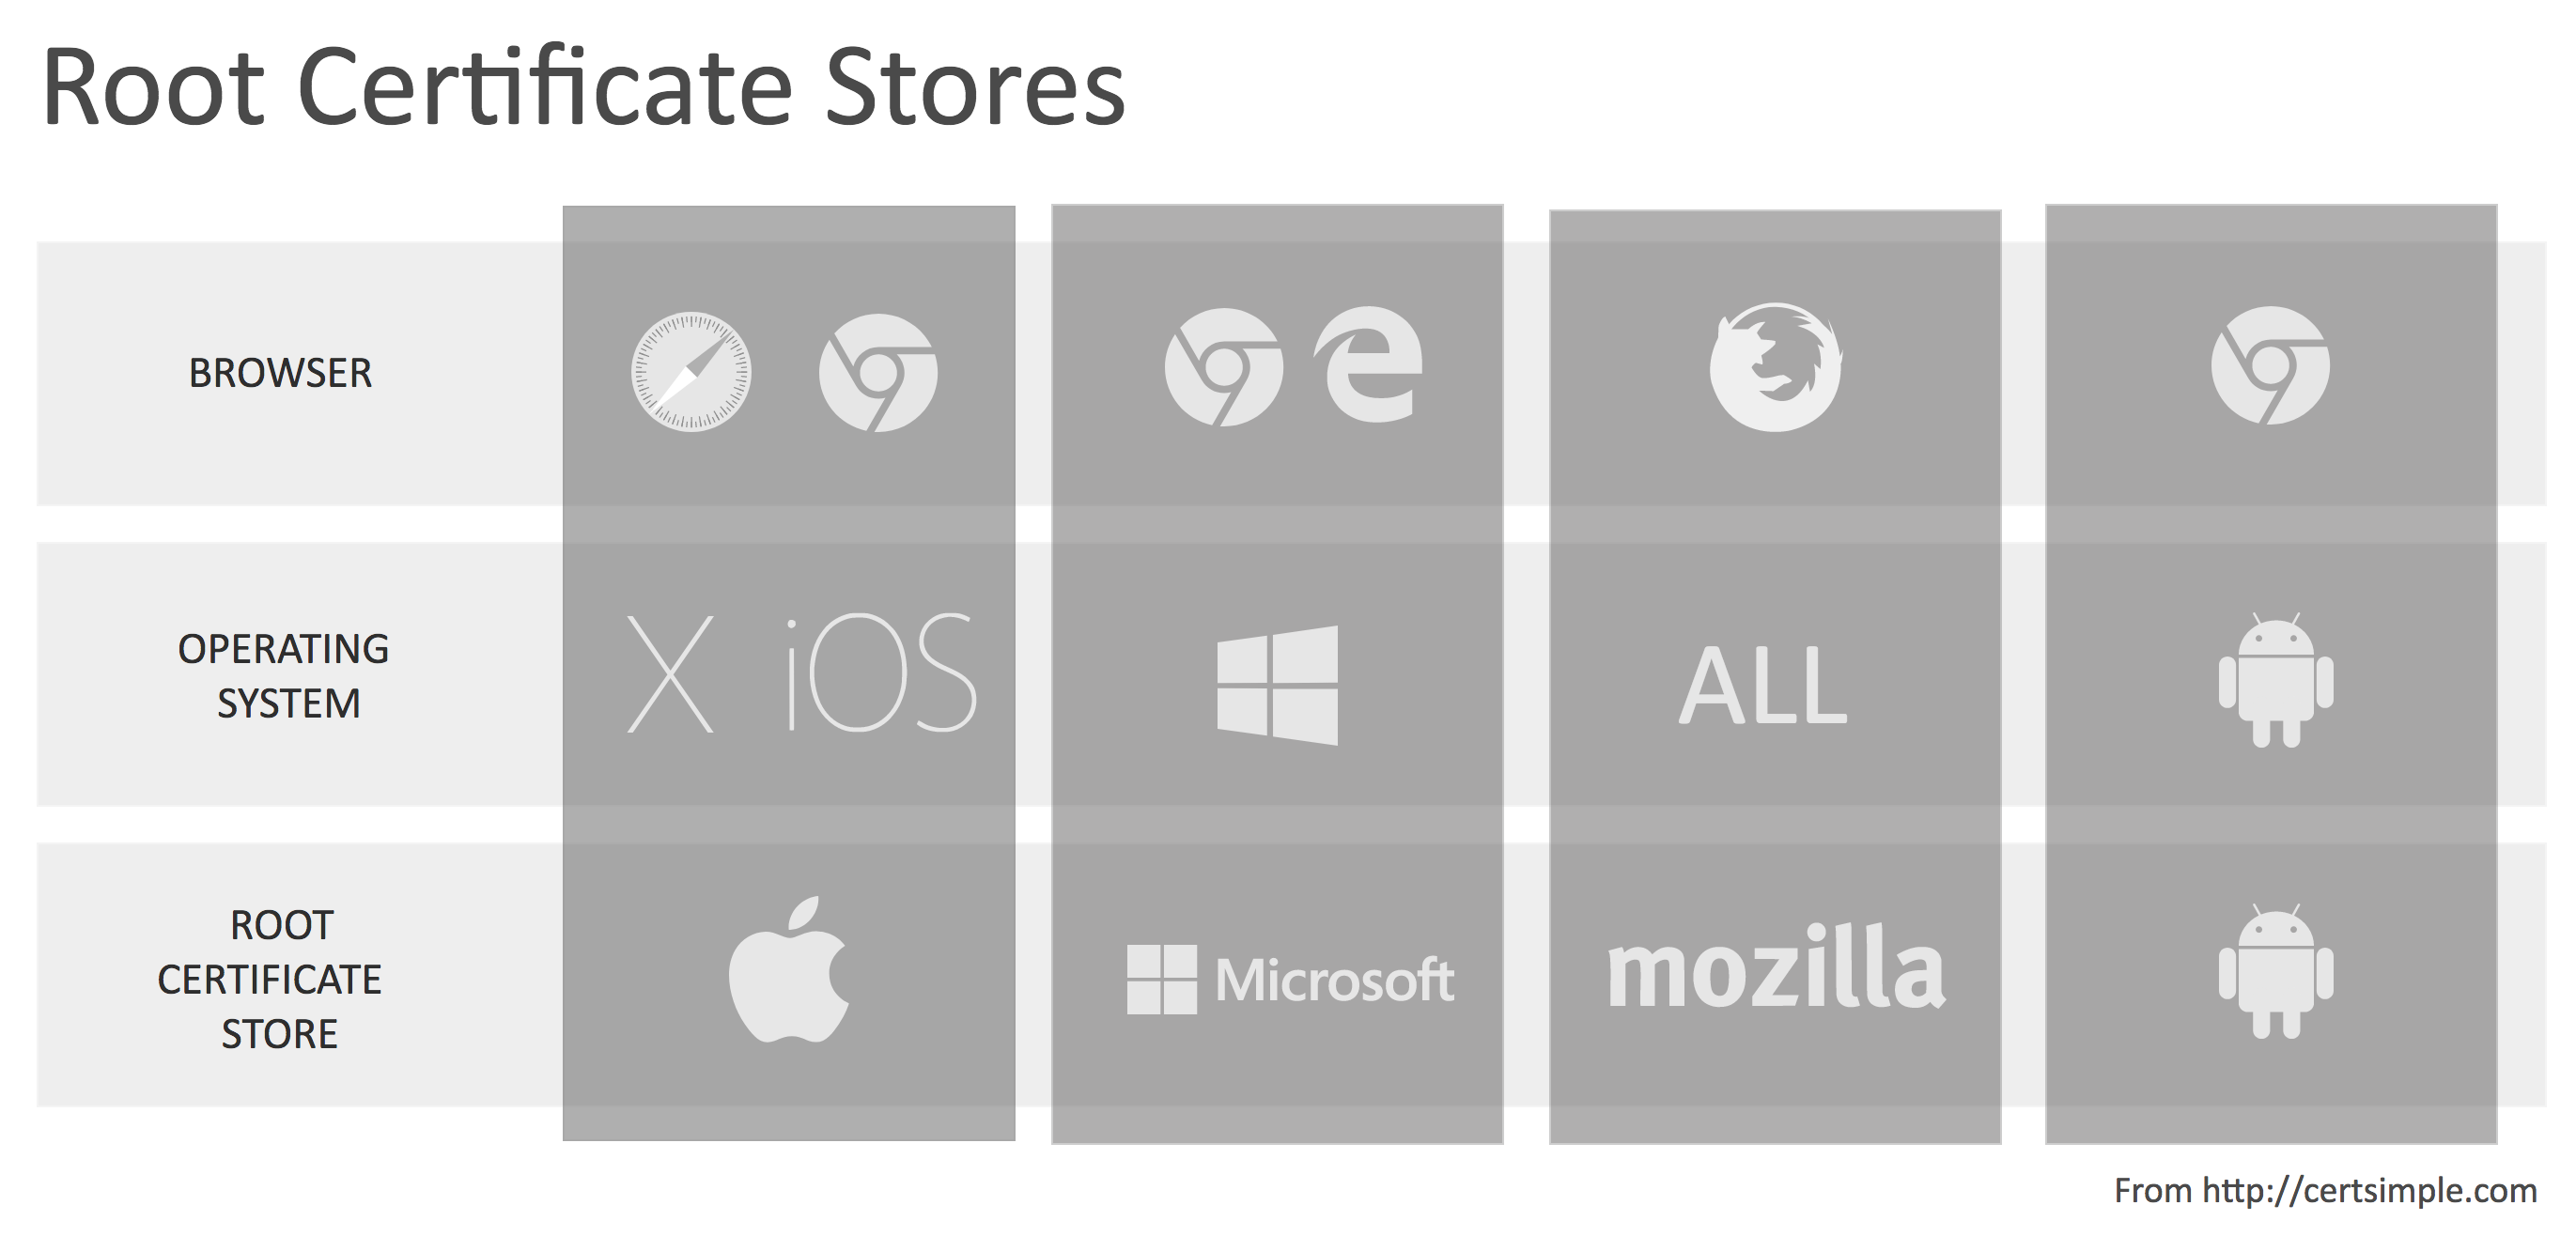
\includegraphics[width=1.0\textwidth]{rootstores-hw5-1642557}
\centering
\caption{From http://certsimple.com}
\label{fig:rootstores}
\end{figure}

Safari supports EV certificates, which require more extensive investigation by certifying agencies \cite{safarisupport}. The macOS Trust Store contains trusted root certificates that are preinstalled with macOS. At the following link you can find a list of trustworthy root certificates: \url{https://support.apple.com/HT208127}. There certificates are divided in three categories:
\begin{itemize}
\item Trusted root certificates that are used to establish a chain of trust with the purpose of verifying other certificates signed by these roots, used for example for web servers.
\item "Always ask" certificates that are not blocked but neither trusted. The user will be prompted wether to trust or not the website using that certificate.
\item "Blocked" certificates are believed to be compromised and will never be trusted.
\end{itemize}
Current versions of Chrome and Safari browsers for macOS use the operating system Trust store and when browsing a website a representation of the site certificate can be retrieved in the following way:
\begin{description}
\item [Safari] To inspect the certificate of a website the user has to look at the address/search bar and to check if a lock icon is present. When the icon is present, clicking on it will open a windows prompting the user to show the certificate, that will be shown after clicking on the \
"Show certificate" button.
\item [Chrome] In Chrome the certificates by default are visible only accessing the developer options of the current website. However the user can manually enable a link for showing the website certificate by issuing the following command in the search bar: \texttt{chrome://flags/\#show-cert-link}; in the resulting page, in the first lines the user can click on an "Enable" option that will add a faster access to the certificate in the browser. After restarting the browser clicking on the specific area in the address bar it is now possible to access the certificate info.
\end{description}

In Mozilla Firefox there's a different certificate trust store that is managed by Mozilla itself. In the last release of Firefox (57.0 Quantum) on macOS, the user can access the information about a certificate by clicking on the security info icon in the address bar and then clicking on the \texttt{More information} button. In this way the user will be able to access a detailed interface to consult and even export the website certificate, as shown in the screenshot in Figure\ref{fig:firefox} (the reader will forgive us for the use of Italian as the system language).

\begin{figure}[h]
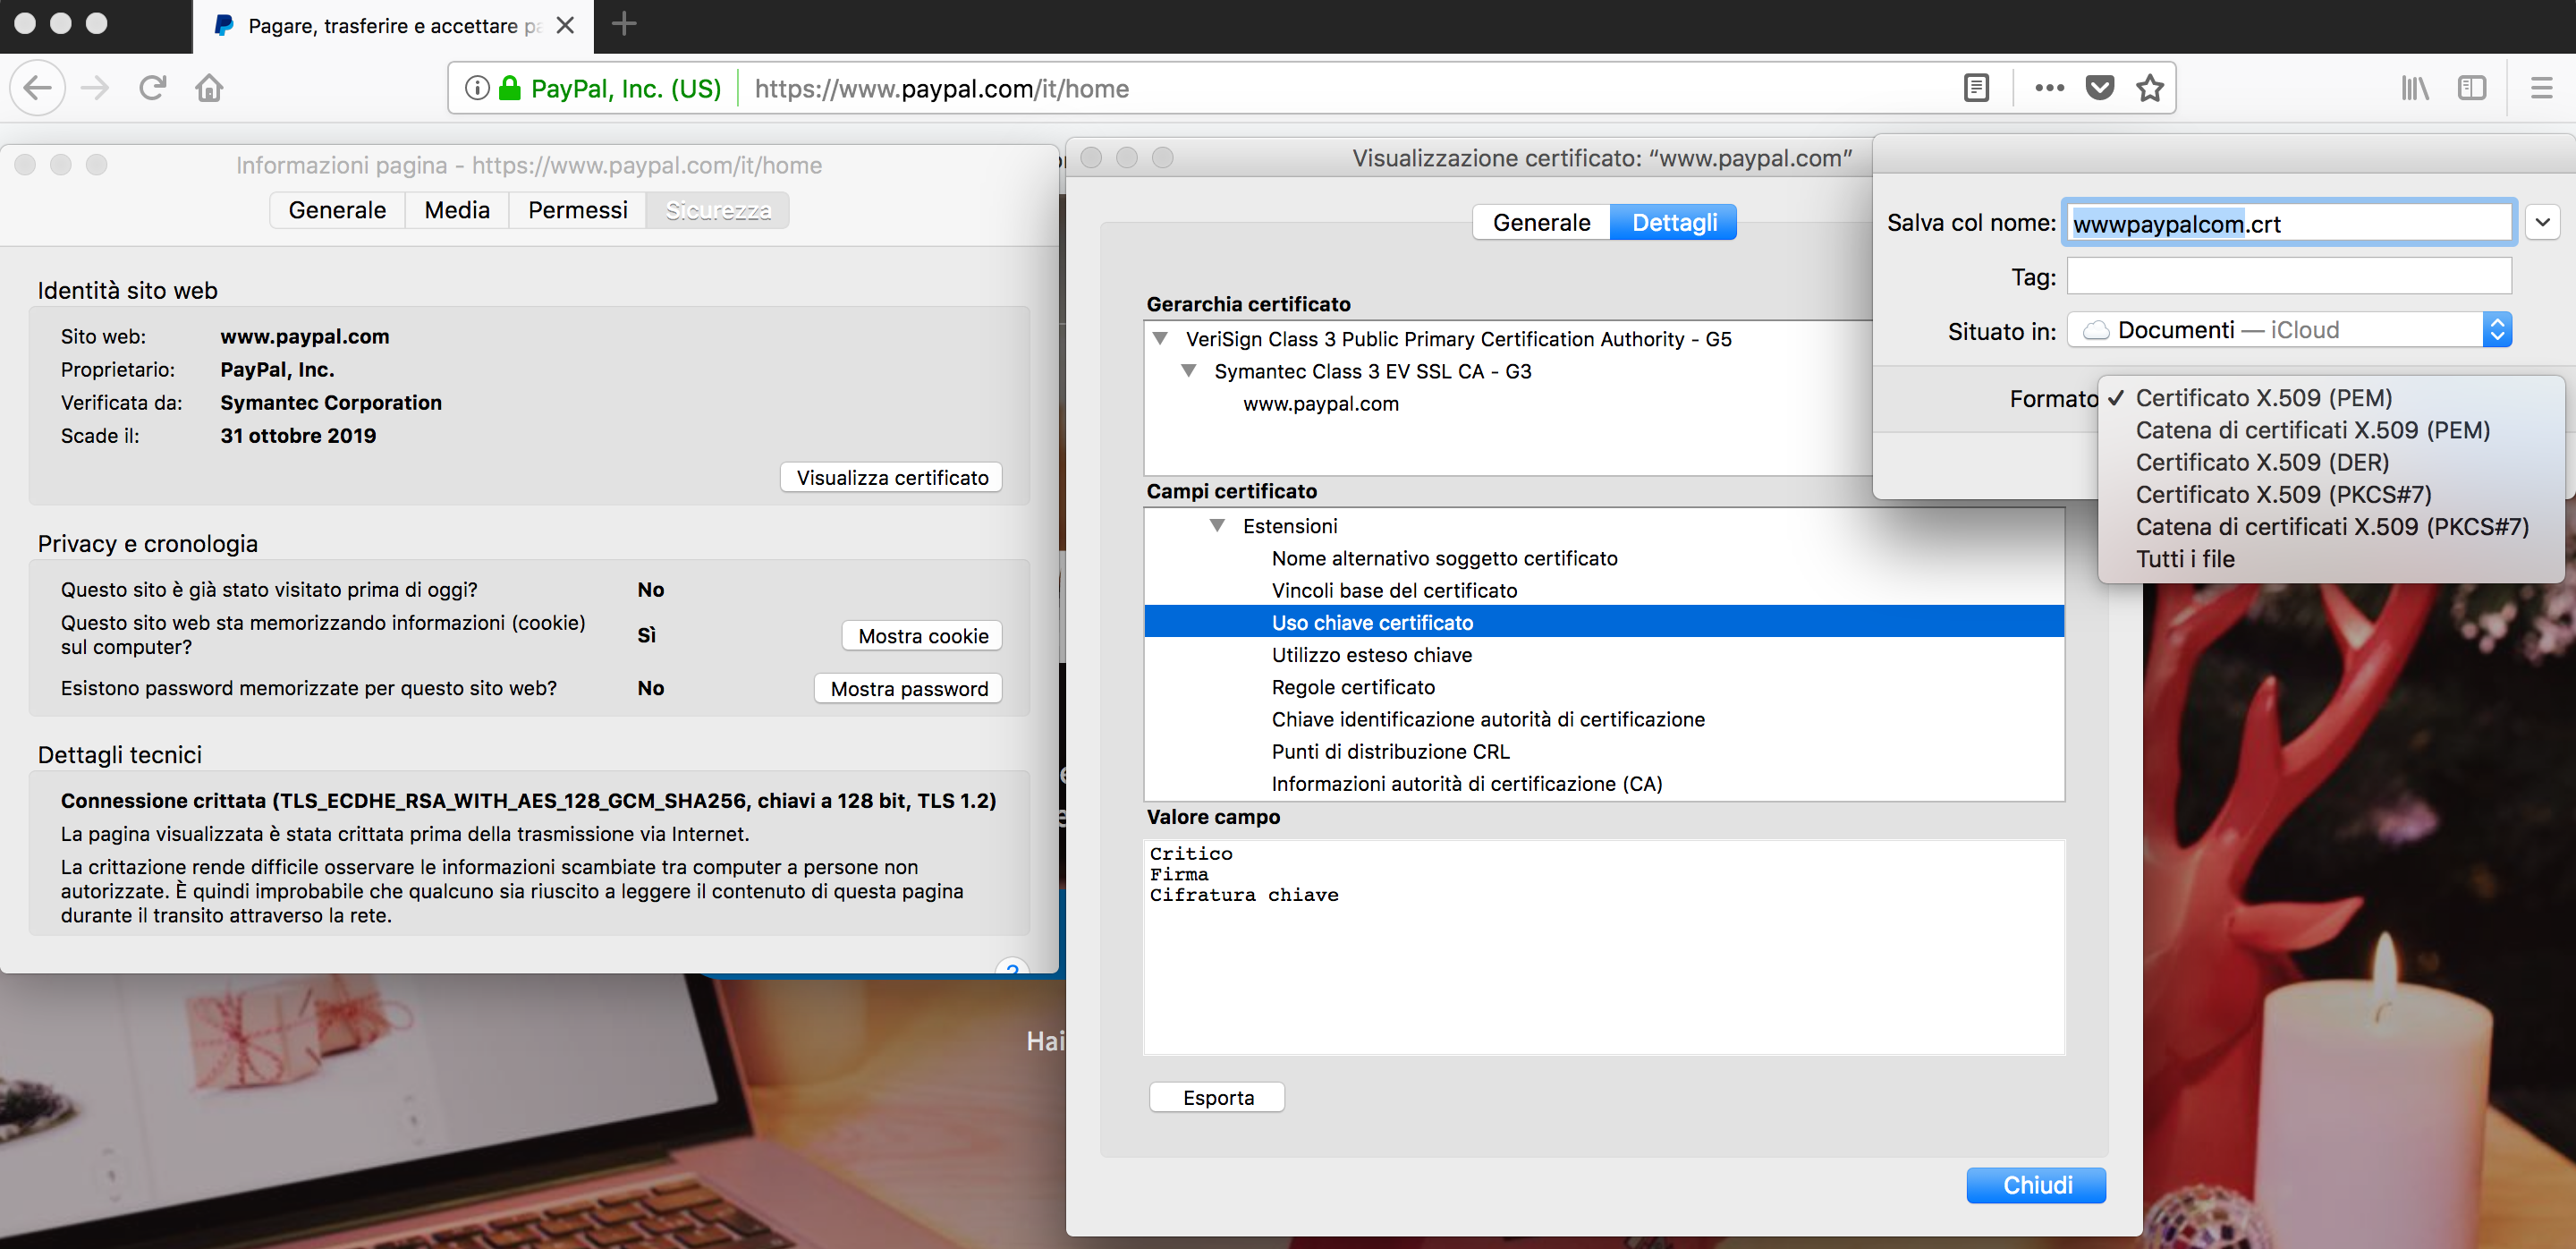
\includegraphics[width=1.0\textwidth]{firefox-hw5-1642557}
\centering
\caption{A screenshot of the certificates interface in Firefox Quantum for macOS.}
\label{fig:firefox}
\end{figure}

Finally we want to just give a quick guide on how to read the certificate of a website when using the Chrome Android application. The procedure is simple but it only visualizes major information about the certificate. We want also to poin out that starting from Android 4.0 (Android ICS/'Ice Cream Sandwich', Android 4.3 'Jelly Bean' and Android 4.4 'KitKat'), system trusted certificates are on the (read-only) system partition in the folder '/system/etc/security/' as individual files. However, users can now easily add their own 'user' certificates which will be stored in '/data/misc/keychain/certs-added'. System-installed certificates can be managed on the Android device in the Settings -- Security -- Certificates -- 'System'-section, whereas the user trusted certificates are managed in the 'User'-section there. Installing new certificates as 'system trusted'-certificates requires more work and requires root access to the device \cite{android}.

\section{Conclusions}
In this work we have seen several information and tips about the usage of digital certificates in the macOS system with the most commonly used browsers like Safari, Chrome and Firefox. We also discussed the basics of digital certificates along with the Certification Authority notion, trying to identificate the main mechanisms behind chains of trust. 

%\clearpage
\nocite{*} % Show all Bib-entries
\bibliography{hw5-1642557} 
\bibliographystyle{plainurl}

\end{document}